\documentclass[11pt, oneside]{scrbook}

\usepackage[english]{babel}

\usepackage[]{handout}
\usepackage{scrhack}
% \setlist{nosep}

\graphicspath{{images/}}

\title{Quantum Cellular Automata}
\subtitle{NIUS Physics (Batch 20) \\ Mid-Term Report \\ Camp: 20.2}
\author{
    Piyush Kumar Singh\thanks{\mailto{pks22ms027@iiserkol.ac.in}} \\ {\large IISER Kolkata} 
    \and
    % Rhythm Anand\thanks{\mailto{rhythm.anand@students.iiserpune.ac.in}} \\ {\large IISER Pune}
    % \and
    Sambuddha Sanyal\thanks{\mailto{sambuddha.sanyal@iisertirupati.ac.in}} \\ {\large IISER Tirupati}
}
\date{
    \today \\
    \vspace{5ex}
    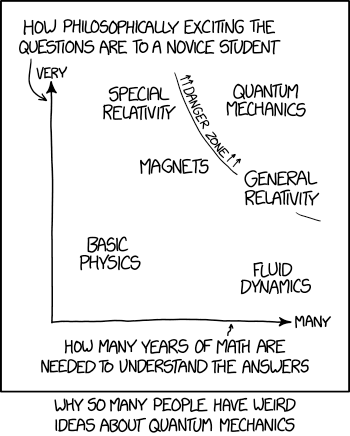
\includegraphics[width = 0.6\textwidth]{quantum-xkcd.png}
}

\changemaincolor{Emerald}
\changesecondcolor{Periwinkle}

% \usepackage{biblatex}
\addbibresource{references.bib}

\hypersetup{
    pdftitle={Quantum Cellular Automata},
    pdfauthor={Piyush Kumar Singh, Rhythm Anand, Sambuddha Sanyal},
    pdfkeywords={physics, cellular automata, quantum cellular automata, thermalization},
    linktocpage=true
}

\begin{document}
\frontmatter
\begin{titlepage}
    \let\newpage\relax%
    \singhtitle
\end{titlepage}

\chapter*{Acknowledgement}
\addcontentsline{toc}{chapter}{Acknowledgement}

{\large\noindent
    This work was supported by the National Initiative on Undergraduate Science (NIUS) undertaken
    by the Homi Bhabha Centre for Science Education, Tata Institute of Fundamental Research
    (HBCSE-TIFR), Mumbai, India. We acknowledge the support of the Department of Atomic
    Energy, Govt. Of India, under Project Identification No. RTI4001.}

\tableofcontents

\mainmatter

\chapter{Introduction}

% \lipsum[1]\cite{Hadeler2017}

Cellular automata are discrete mathematical models used to simulate complex systems. John von Neumann first introduced the concept \cite{Neumann1966} in 1966. In 1970, an article written by Martin Gardner \cite{Gardner1970} introduces us to a compelling use case of this abstract concept, ``The Game of Life,'' invented by J. H. Conway.

% In classical cellular automata, the system is divided into discrete cells arranged in a grid. Each cell can be in one of a finite number of states. The state of a cell is typically updated over discrete time steps according to a set of rules based on the states of its neighboring cells.

In a conference in 1982, R. P. Feynman expressed his view (or dream) of using `Quantum Physics' in computers \cite{Feynman1982} to simulate complex physical systems using the idea of density matrix (proposed by Neumann in 1955 \cite{Neumann2018}); building on this idea Feynman introduced the world to a weird collaboration named ``Quantum Cellular Automata'' (QCA) in an article published in 1986 \cite{Feynman1986}.

And there are multiple reasons why we should care about QCAs. First, this is part of a broad field of `Quantum Information Processing,' any development in QCA may help us understand how we can harness quantum properties for computation. Second, the classical systems exhibit some new emergent behaviors, so we want to know if we can also have these emergent behaviors in QCAs.

% When this abstract concept is combined with seemingly weird notions of `Quantum Mechanics,' we get Quantum Cellular Automata (QCA).

Also, in the later part of the discussion, we will see the application of these `discrete' quantum systems (in the form of ``\impt{Random Quantum Circuits}''\cite{Fisher2023}), explaining some of the various emergent properties like:
\begin{enumerate}[(a), noitemsep]
    \item Periodic Fidelity,
    \item Information spread (encoded as \emph{Operator Spread}).
\end{enumerate}

\section{Cellular Automata}

A cellular automaton (CA) is a group of ``coloured'' cells on a predetermined-shaped grid that follows a set of rules depending on nearby cell states to evolve over many discrete time steps. After that, the rules are applied repeatedly for as many time steps as needed.

It turned out that reaction-diffusion systems, biological pattern development, fluid flows, and traffic models are only a few real-world uses for CAs. Lattice gas cellular automata are a specific type of CA used to simulate fluid dynamics. The Navier-Stokes equation can be obtained by selecting the appropriate model. Lattice Boltzmann models have taken their place, using continuous functions at the lattice locations rather than discrete variables. More aspirationally, CAs have been proposed as discrete physics models with many desirable characteristics, such as dynamical homogeneity and localization. But, while this is a fascinating idea, physics is ultimately quantum, and CAs cannot adequately represent, e.g., Bell inequality violation, which occurs from quantum entanglement.

Before giving a formal definition, let's look at an example:
\begin{example}[Rule Number 110]
    \label{eg:rule110}
    Consider a one-dimensional array of bits (\ie cells having two states, namely `0' or `1'). The update rule of a bit is dependent on the initial state of that bit as well as the state of its neighboring bits. The rule can be summarized as follows:
    \begin{table}[H]
        \centering
        \begin{tabular}{ | c | c | c | c | c | c | c | c | c | }
            \hline
            Initial state of a bit and its neighbours & 111 & 110 & 101 & 100 & 011 & 010 & 001 & 000 \\
            \hline
            New state of middle bit                   & 0   & 1   & 1   & 0   & 1   & 1   & 1   & 0   \\
            \hline
        \end{tabular}
        \caption{Update rule for a \textit{one}-dimensional CA}
        \label{tab:rule110}
    \end{table}
    We named this update rule as \verb|Rule 110| because if you treat the last row of the table as a binary number, it converts to 110 in the decimal system. This CA can simulate a Turing machine efficiently (with only polynomial overhead).
    \begin{figure}[H]
        \centering
        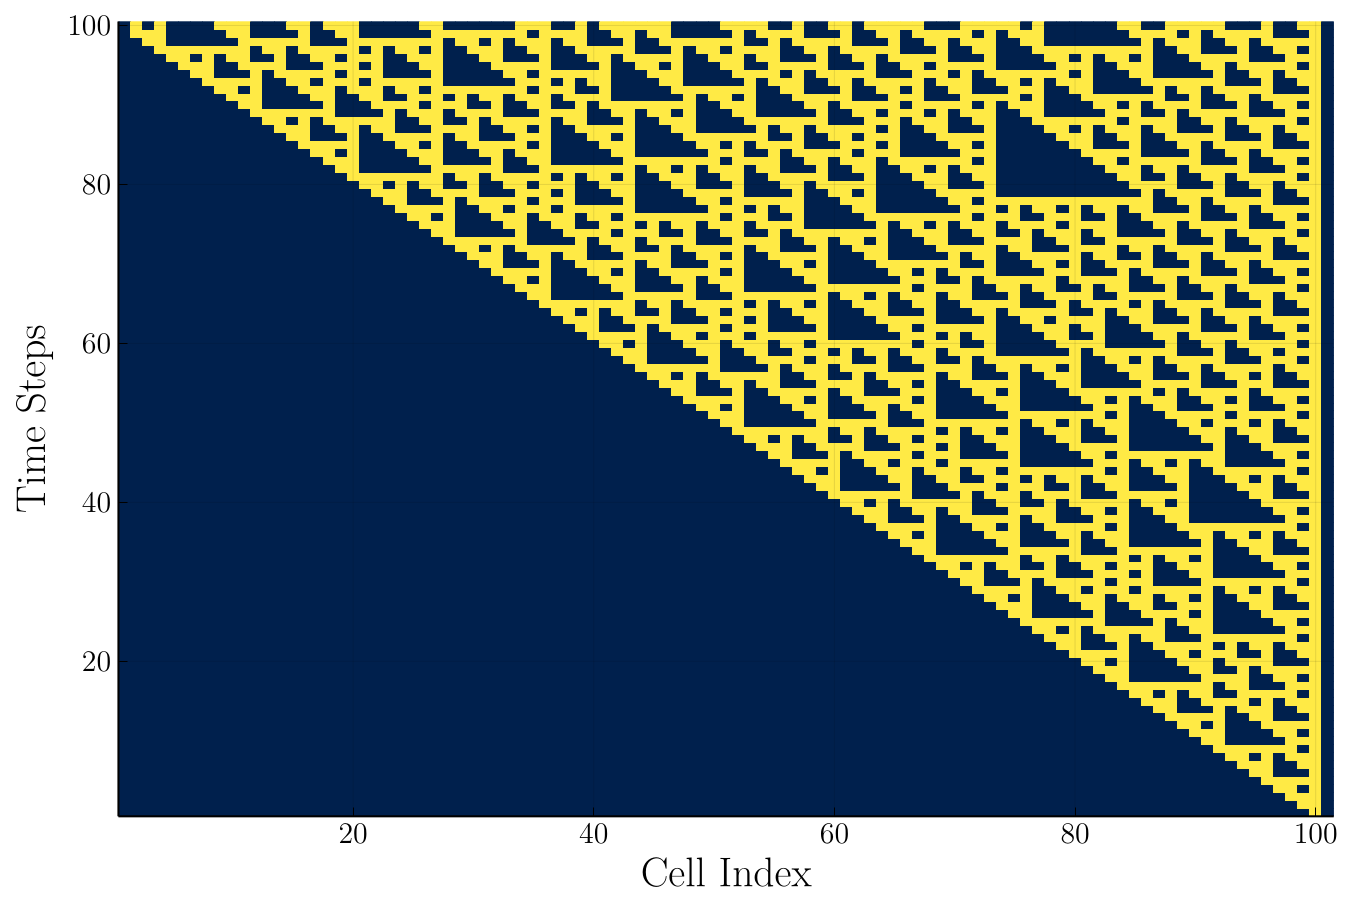
\includegraphics[width = 0.7\textwidth]{rule110_cellular_automaton.png}
        \caption{An example of a CA evolution for the rule 110 CA, with time going up. Bits with value 1 are
            represented by the yellow squares, while blue squares represent 0.}
        \label{fig:rule110}
    \end{figure} \noindent

\end{example}

\begin{definition}[Cellular Automata]
    A Cellular Automaton is a 4-tuple \(\qty(L, \Sigma, \mathcal{N}, f)\) consisting of a $d$-dimensional lattice of cells indexed by integers, $L = \Z^d$, a finite set $\Sigma$ of cell states, a finite neighborhood scheme $\mathcal{N} \subseteq \Z^d$, and a local transition function $f: \Sigma^{\mathcal{N}} \to \Sigma$.
\end{definition}

% There are a few unique characteristics of this local transition function \(f\). Consider a cell \(x \in L\)
To better understand this local transition function \(f\), consider a cell \(x \in L\). This function takes the state of the neighbours of \(x\) as the argument, which is indexed by the set \(\mathcal{N}\) at the current time \(t \in \Z\) to spit out the state of cell $x$ at time $t + 1$.

\noindent This observation points us towards two important properties of cellular automata that will help us understand why CAs are very helpful in simulating certain systems:

\begin{itemize}
    \item cellular automata are \vocab{space-homogeneous} \ie the local transition function performs the same function at each cell.
    \item Also, cellular automata are \vocab{time-homogeneous} \ie the local transition function does not depend on the time step $t$.\footnote{We will review these properties in detail in \cref{ssec: locality,ssec: universality}}
\end{itemize}

\noindent We can define the current state of the lattice (or CA) as a \emph{configuration} \(C \in \Sigma^{L}\), which has the information about the state of each cell at time \(t\). Now, using this idea, we can define a `\emph{global}' transition function \(F: \Sigma^{L} \to \Sigma^{L}\), which acts on the entire latter rather than on individual cells and spits out another configuration \(C'\) for the lattice at time \(t+1\).

\begin{remark}[Revisiting Rule 110]
    Observe the \cref{eg:rule110}; we can fit this scenario in the definition. In this case \(L = \Z\), \(\Sigma = \qty{0, 1}\), for $i^{\text{th}}$ cell \(\mathcal{N} := \qty{i-1,~ i,~ i+1}\) and \(f\) is defined according to the update rule specified in \cref{tab:rule110}.
\end{remark}

\subsection{Characteristics of Cellular Automata}

\subsection{Locality} \label{ssec: locality}

\subsection{Universality} \label{ssec: universality}
\lipsum[3]

\section{Quantum Cellular Automata}
\lipsum[5-15]


\chapter{Random Quantum Circuits}

\appendix
\chapter{Notations}
\section{Hello}

\backmatter
\printbibliography[heading=bibintoc, title=Bibliography]

\end{document}